\documentclass{article}
\usepackage{amsmath,amssymb,amsthm,kotex,mdframed,paralist}

\newcounter{num}
\newcommand{\defi}[1]
{\bigskip\noindent\refstepcounter{num}\textbf{정의 \arabic{num}) #1}\par}
\newcommand{\theo}[1]
{\bigskip\noindent\refstepcounter{num}\textbf{정리 \arabic{num}) #1}\par}
\newcommand{\exam}[1]
{\bigskip\noindent\refstepcounter{num}\textbf{예시 \arabic{num}) #1}\par}
\newcommand{\prob}[1]
{\bigskip\noindent\refstepcounter{num}\textbf{문제 \arabic{num}) #1}\par}
\newcommand{\summ}[1]
{\bigskip\noindent\refstepcounter{num}\textbf{요약 \arabic{num}) #1}\par}

\renewcommand{\figurename}{그림}
\renewcommand{\proofname}{증명)}
\newcommand{\sol}{\par\bigskip\noindent{\bfseries풀이)}\par}
%\newcommand{\ans}[1]{\par{\raggedleft답)#1}\par}

%\newcommand{\ans}[1]{
%\raggedleft
%답)
%#1
%
%}


%%%
\begin{document}

\title{영석 : 09 기말고사(1학년 1학기) 대비 개념 요약}
\author{}
\date{\today}
\maketitle
\tableofcontents
\newpage

%%
\section{여러 가지 부등식}
\summ{}
\begin{enumerate}
\item
부등식의 양변에 같은 값을 더하거나 빼더라도 부등호의 방향은 바뀌지 않는다.
\item
부등식의 양변에 같은 값을 곱하거나 나눌 때에는, 곱하거나 나누는 수가 양수이면 부등호의 방향이 바뀌지 않고, 음수이면 부등호의 방향이 바뀐다.
\item
양수 \(a\)에 대해,
\begin{enumerate}
\item
\(|x|<a\)이면 \(-a<x<a\)이다.
\item
\(|x|>a\)이면 \(x<-a\) 또는 \(x>a\)이다.
\end{enumerate}
\item
이차부등식의 해는 다음과 같이 구한다(\(a>0\)).
\bigskip

\noindent
{\footnotesize
\begin{tabular}{p{0.24\textwidth}|p{0.24\textwidth}|p{0.24\textwidth}|p{0.24\textwidth}}
\hline
&\(D>0\)		&\(D=0\)	&\(D<0\)\\
\hline
\(y=ax^2+bx+c\)의 그래프
&\raisebox{-.5\height}{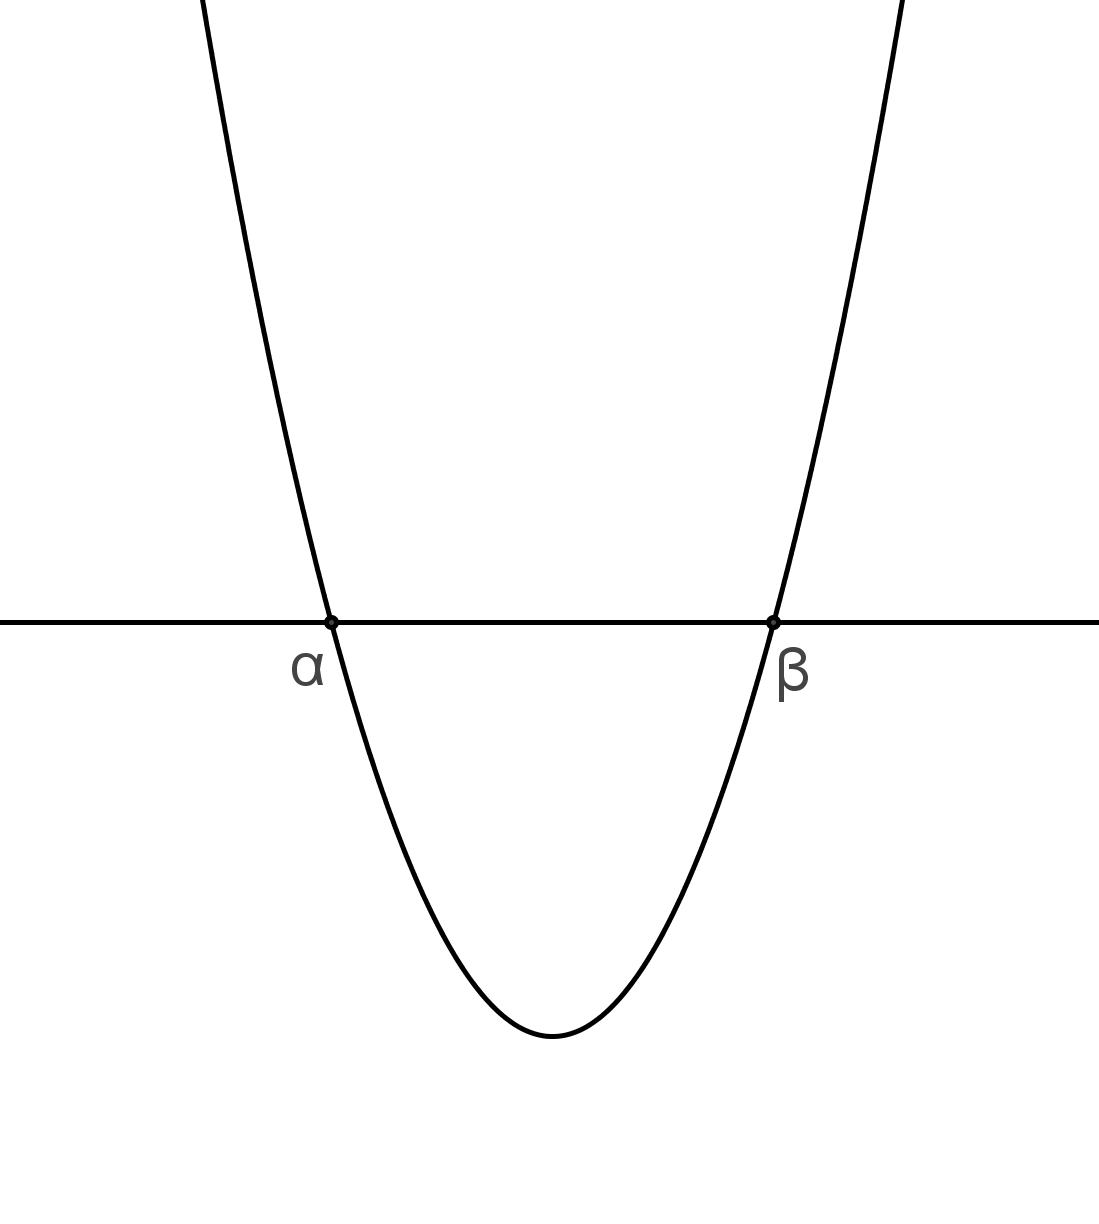
\includegraphics[width=0.24\textwidth]{1}}
&\raisebox{-.5\height}{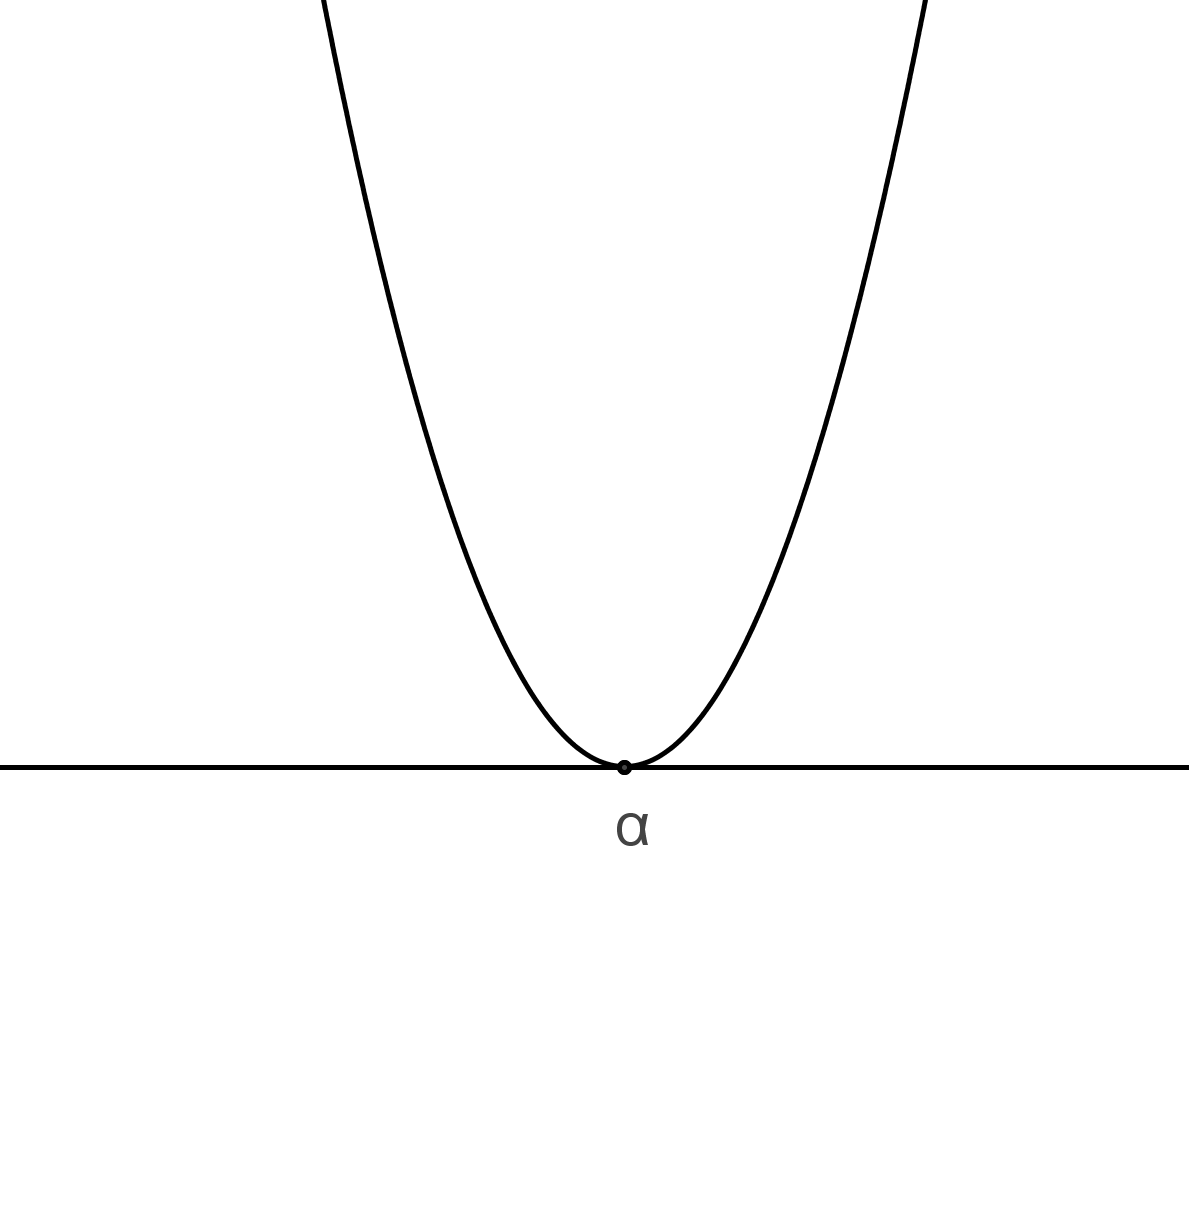
\includegraphics[width=0.24\textwidth]{2}}
&\raisebox{-.5\height}{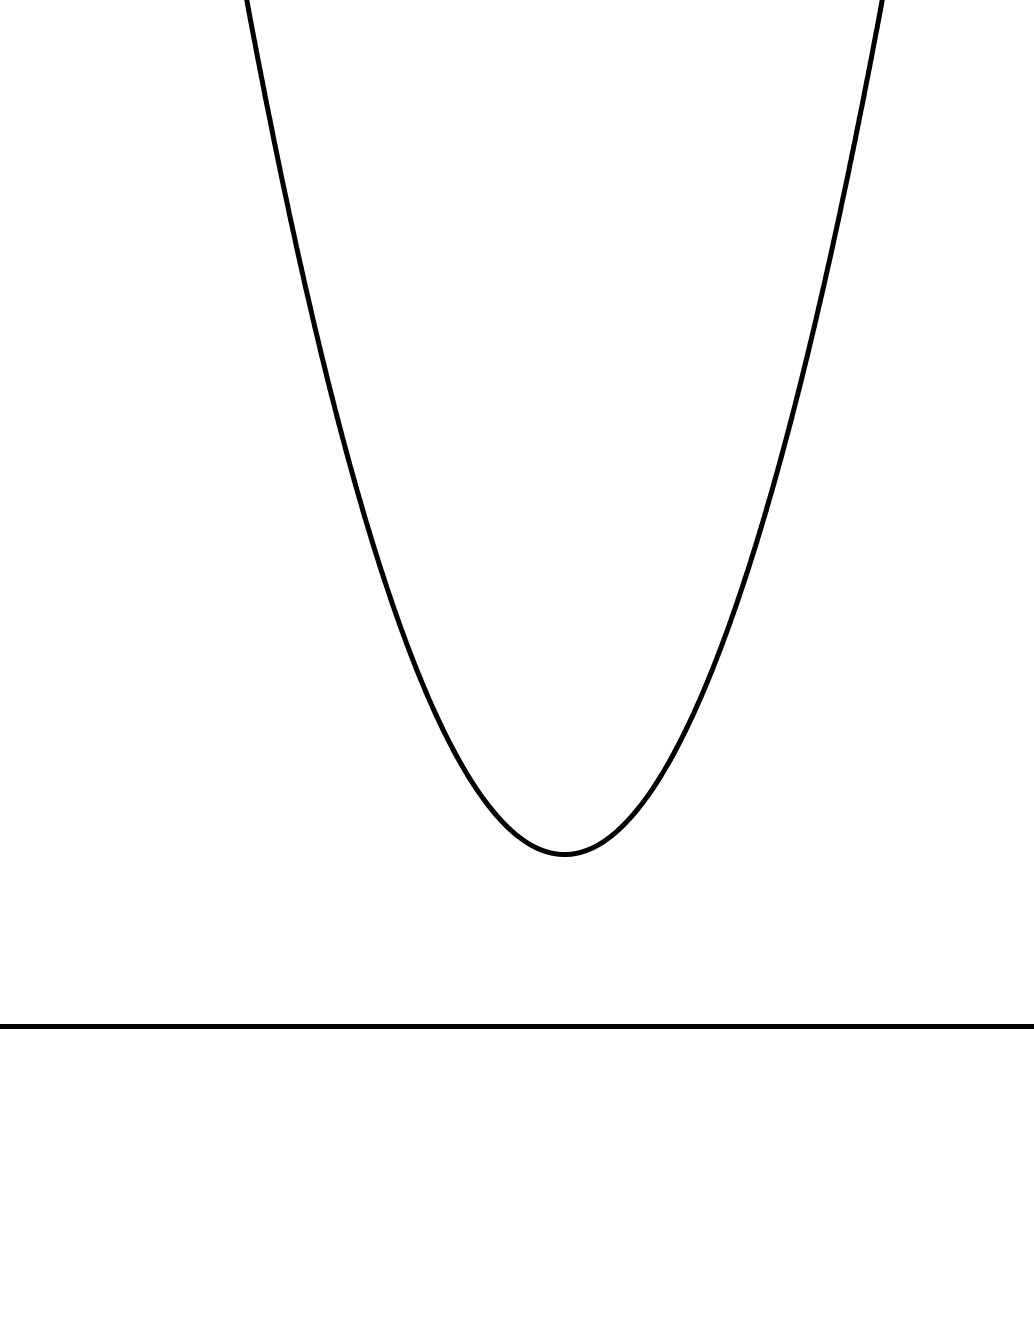
\includegraphics[width=0.24\textwidth]{3}}\\
\hline
\(ax^2+bx+c>0\)의 해
&\(x<\alpha\) 또는 \(x>\beta\)		&\(x\neq\alpha\)인 모든 실수	&모든 실수\\\hline
\(ax^2+bx+c\ge0\)의 해
&\(x\le\alpha\) 또는 \(x\ge\beta\)	&모든 실수					&모든 실수\\\hline
\(ax^2+bx+c<0\)의 해
&\(\alpha<x<\beta\)				&없다.					&없다.\\\hline
\(ax^2+bx+c\le0\)의 해
&\(\alpha\le x\le\beta\)			&\(x=\alpha\)				&없다.\\\hline
\end{tabular}
}\end{enumerate}

%%
%\exam{}
%다음 부등식을 풀어라.\\
%(1) \(3x<9\)\\
%(2) \(6-3x\ge2(x+1)\)
%
%\sol
%(1) 양변을 \(3\)으로 나누면 \(x<3\)이다.
%
%(2) 우변을 전개하면 \(6-3x\ge2x+2\)이고, 양변에서 \(6\)을 빼면 (\(6\)을 이항하면) \(-3x\ge2x-4\)이며, 다시 양변에서 \(2x\)를 빼면 \(-5x\ge-4\)가 된다.
%마지막으로 양변을 \(-5\)로 나누면 \(x\le\frac45\)이다.
%
%%
%\prob{}
%다음 부등식을 풀어라.\\
%(1) \(3x-2<13\)\\
%(2) \(x+2\ge-2x+5\)

%\ans{11}
%
%{
%\raggedleft
%답)
%This is a paragraph. I'm testing alignments in \LaTeX
%
%}
%
%{
%\raggedleft
%This is a paragraph. I'm testing alignments in \LaTeX
%
%}

%%
%\exam{}
%부등식 \(|x-2|<3\)을 풀어라.
%\sol
%\(-3<x-2<3\)이 성립한다.
%이는 \(-3<x-2\)와 \(x-2<3\)이 성립한다는 뜻이다.
%각각을 정리하면 \(x>-1\), \(x<5\)가 되므로 \(-1<x<5\)이다.
%
%%
%\exam{}
%다음 이차부등식을 풀어라.\\
%(1) \(x^2-2x-3>0\)\\
%(2) \(x^2+2x+2\le0\)
%\sol
%(1)
%\(D=(-2)^2-4\cdot1\cdot(-3)>0\)이므로 좌변을 \((x-\alpha)(x-\beta)\)의 꼴로 만들 수 있다.
%좌변을 인수분해하면 \((x-3)(x+1)\)이고, 그래프를 그리면 그림 \ref{y=x^2-2x-3}과 같이 나타나므로 \(x<-1\) 또는 \(x>3\)이다.
%
%\begin{figure}[h!]
%\center
%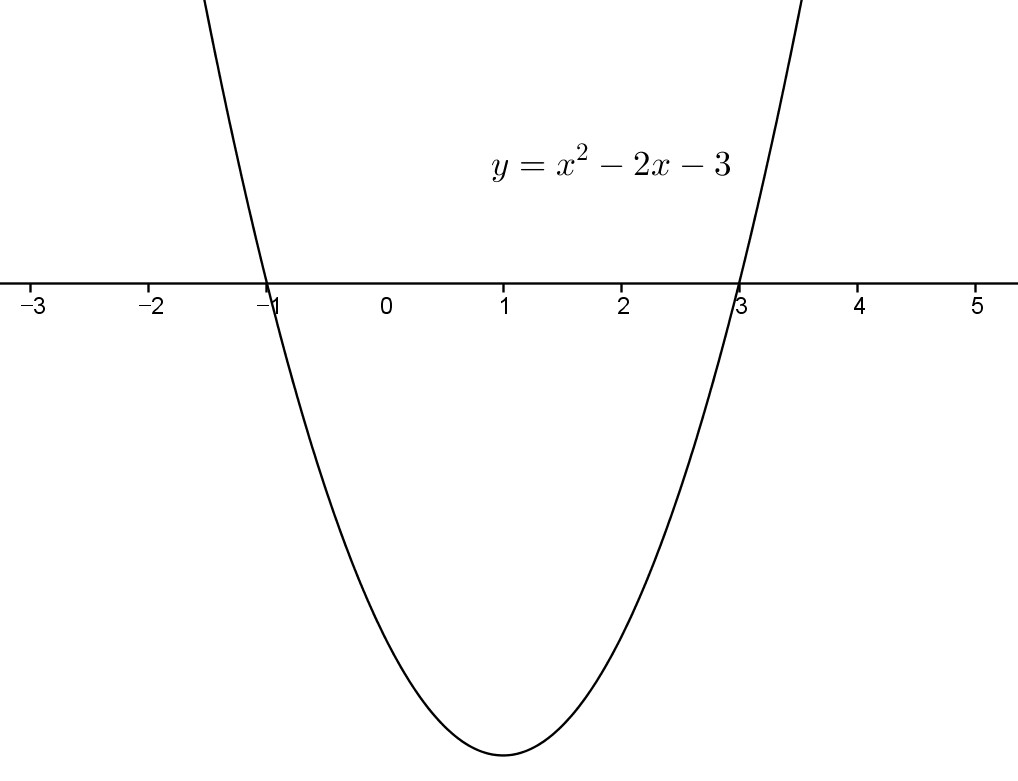
\includegraphics[width=0.4\textwidth]{y=x^2-2x-3}
%\caption{\(y=x^2-2x-3\)의 그래프}
%\label{y=x^2-2x-3}
%\end{figure}
%\noindent
%
%(2) \(D=2^2-4\cdot1\cdot2<0\)이므로 \(y=x^2+2x+2\)의 그래프는 그림 \ref{y=x^2+2x+2}와 같다.
%따라서 해는 없다.
%
%\begin{figure}[h!]
%\center
%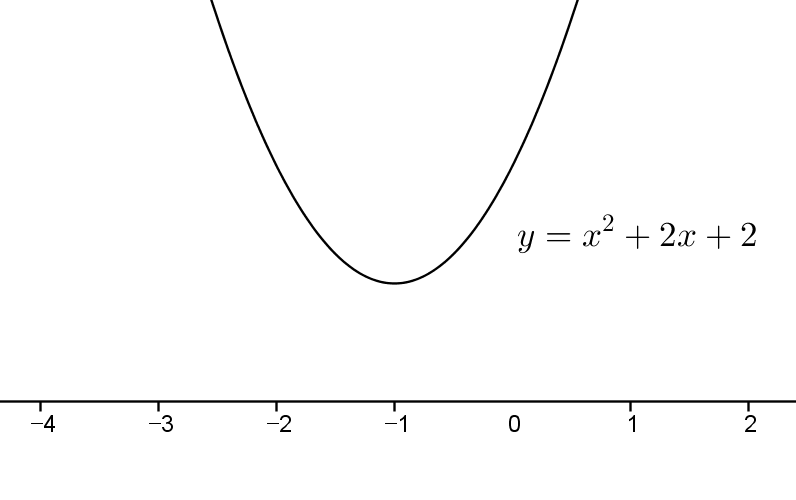
\includegraphics[width=0.4\textwidth]{y=x^2+2x+2}
%\caption{\(y=x^2+2x+2\)의 그래프}
%\label{y=x^2+2x+2}
%\end{figure}

%%
\section{평면좌표}

%
\summ{}
\begin{enumerate}
\item
수직선 상의 두 점 \(A(x_1)\), \(B(x_2)\) 사이의 거리는 \(|x_1-x_2|\)이다.
\item
좌표 평면 위의 두 점 \(A(x_1,y_1)\), \(B(x_2,y_2)\) 사이의 거리는 \(\sqrt{(x_1-x_2)^2+(y_1-y_2)^2}\)이다.
\item
수직선 상의 두 점 \(A(x_1)\), \(B(x_2)\)에 대해 \(m:n\) 내분점 \(P\)와 외분점 \(Q\)의 좌표는 \(P=(\frac{mx_2+nx_1}{m+n})\), \(Q=(\frac{mx_2-nx_1}{m-n})\) 이다.
\item
좌표평면 상의 두 점 \(A(x_1,y_1)\), \(B(x_2,y_2)\)에 대한 \(m:n\) 내분점 \(P\)와 외분점 \(Q\)의 좌표는 \(P=(\frac{mx_2+nx_1}{m+n},\frac{my_2+ny_1}{m+n})\), \(Q=(\frac{mx_2-nx_1}{m-n},\frac{my_2-ny_1}{m-n})\) 이다.
\item
두 점 \(A(x_1,y_1)\), \(B(x_2,y_2)\)가 이루는 선분 \(AB\)의 중점 \(M\)의 좌표는
\(M=(\frac{x_1+x_2}2,\frac{y_1+y_2}2)\)
이다.
\item
세 점 \(A(x_1,y_1)\), \(B(x_2,y_2)\), \(C(x_3,y_3)\)가 이루는 삼각형 \(ABC\)의 무게중심 \(G\)의 좌표는
\(G=(\frac{x_1+x_2+x_3}3,\frac{y_1+y_2+y_3}3)\)
이다.
\end{enumerate}

%%
%\exam{}
%다음 두 점 사이의 거리를 구하여라.\\
%(1) \(A(0,0)\), \(B(3,4)\)\\
%(2) \(A(-1,2)\), \(B(11,7)\)
%
%\sol
%(1) \(\overline{AB}=\sqrt{(0-3)^2+(0-4)^2}=\sqrt{25}=5\)
%
%(2) \(\overline{AB}=\sqrt{(-1-11)^2+(2-7)^2}=\sqrt{169}=13\)
%
%%
%\exam{}
%두 점 \(A(5,3)\), \(B(-2,1)\)에 대하여 다음 점의 좌표를 구하여라.\\
%(1) 선분 \(AB\)를 \(1:2\)로 내분하는 점\\
%(2) 선분 \(AB\)를 \(1:2\)로 외분하는 점
%
%\sol
%(1) 내분점을 \(P\)라고 하면
%\(P=(\frac{1\cdot(-2)+2\cdot5}{1+2},\frac{1\cdot1+2\cdot3}{1+2})=(\frac83,\frac73)\)
%
%(2) 외분점을 \(Q\)라고 하면
%\(Q=(\frac{1\cdot(-2)-2\cdot5}{1-2},\frac{1\cdot1-2\cdot3}{1-2})=(12,5)\)
%
%%
%\exam{}
%세 점 \(A(-3,5)\), \(B(1,4)\), \(C(2,-2)\)를 꼭짓점으로 하는 삼각형 \(ABC\)의 무게중심의 좌표를 구하여라.
%
%\sol
%무게중심을 \(G\)라고 하면 \(G=(\frac{(-3)+1+2}3,\frac{5+4+(-2)}3)=(0,\frac73)\) 이다.

%%
\section{직선의 방정식}

%
\summ{}
\begin{enumerate}
\item
\(y=mx+n\)은 기울기가 \(m\)이고 \(y\)절편이 \(n\)인 직선이다.
하지만 평면 위의 모든 직선이 \(y=mx+n\)꼴로 표현될 수는 없다.
\(y\)축에 평행한 \(x=1\)과 같은 직선은 \(y=mx+n\)꼴로 표현할 수 없기 때문이다.
따라서 \(ax+by+c=0\)으로 직선을 표시하면 모든 형태의 직선의 방정식을 포괄할 수 있다.
\item
기울기가 \(m\)이고 한 점 \((x_1,y_1)\)을 지나는 직선의 방정식은 \(y-y_1=m(x-x_1)\)이다.
\item
\(x_1\neq x_2\)일 때, 두 점\((x_1,y_1)\), \((x_2,y_2)\)을 지나는 직선의 방정식은 \(y-y_1=\frac{y_2-y_1}{x_2-x_1}(x-x_1)\)이다. 
\item
두 직선 \(y=mx+n\)과 \(y=m'x+n'\)에 대해
\begin{enumerate}
\item
\(m=m'\), \(n=n'\)이면 두 직선은 일치한다.
\item
\(m=m'\), \(n\neq n'\)이면 두 직선은 평행하다.
\item
\(m\neq m'\)이면 두 직선은 한 점에서 만난다.
\item
\(mm'=-1\)이면 두 직선은 서로 수직이다.
\end{enumerate}
\item
점 \(A(x_1,y_1)\)와 직선 \(l:ax+by+c=0\) 사이의 거리는 \(A\)에서 \(l\)에 그은 수선의 길이로 정의하며(그림 \ref{line-point}), 그 값 \(d\)는 다음과 같다.
\[d=\frac{|ax_1+by_1+c|}{\sqrt{a^2+b^2}}.\]
\end{enumerate}

\begin{figure}[h]
\center
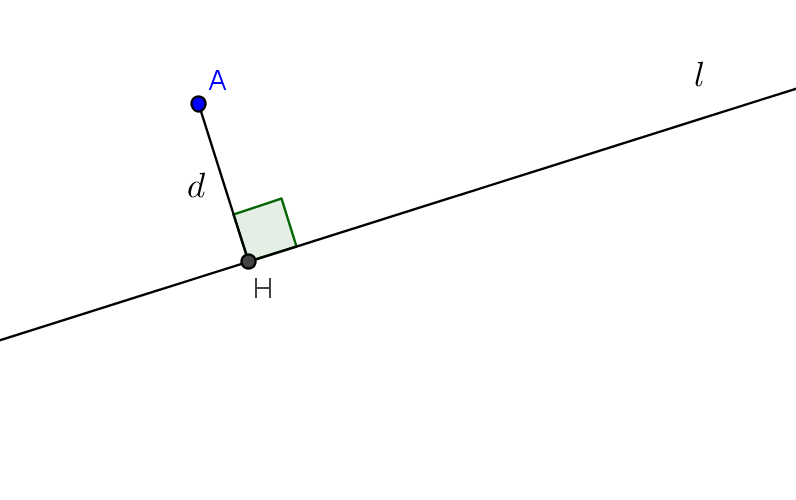
\includegraphics[width=0.5\textwidth]{line-point}
\caption{점과 직선 사이의 거리}
\label{line-point}
\end{figure}

%%
\section{원의 방정식}

%
\summ{}
\begin{enumerate}
\item
중심이 \(C(a,b)\)이고 반지름이 \(r\)인 원의 방정식은 \((x-a)^2+(y-b)^2=r^2\)이다.
\item
원 \(x^2+y^2=r^2\)에 접하고 기울기가 \(m\)인 접선의 방정식은 \(y=mx\pm r\sqrt{m^2+1}\)이다.
\item
원 \(x^2+y^2=r^2\) 위의 점 \((x_1,y_1)\)에서 그은 접선의 방정식은 \(x_1x+y_1y=r^2\)이다.
\end{enumerate}

%
\summ{원과 직선 사이의 위치관계}
\begin{enumerate}
\item
직선과 원의 교점은 최대 두 개까지 존재할 수 있다.
교점이 2개면 이 직선을 할선이라고 부른다,
교점이 1개면 이 직선을 접선이라고 부르며, 이때의 교점을 접점이라고 부른다.
\item
원 \(x^2+y^2=r^2\)과 직선 \(ax+by+c=0\)의 교점의 개수는 다음 두 방법을 사용해 판별할 수 있다(그림 \ref{line-circle}).
\begin{enumerate}
\item
판별식을 이용하는 방법 :
두 도형 사이의 교점의 갯수는 두 식으로 만들어지는 연립방정식의 해의 갯수와 같으므로, 두 식을 연립하여 푼다.
연립할 때에 나타나는 이차방정식에서
(1) \(D>0\)이면 교점의 갯수가 두 개이고,
(2) \(D=0\)이면 교점의 갯수가 한 개이며,
(3) \(D<0\)이면 교점이 없다.
\item
점과 직선사이의 거리를 이용하는 방법 :
원의 중심과 직선사이의 거리를 \(d\)라고 하자.
(1) \(d<r\)이면  교점의 갯수가  두 개이고,
(2) \(d=r\)이면 교점의 갯수가 한 개이며,
(3) \(d<r\)이면 교점이 없다.
\end{enumerate}
\end{enumerate}

\begin{figure}[h]
\center
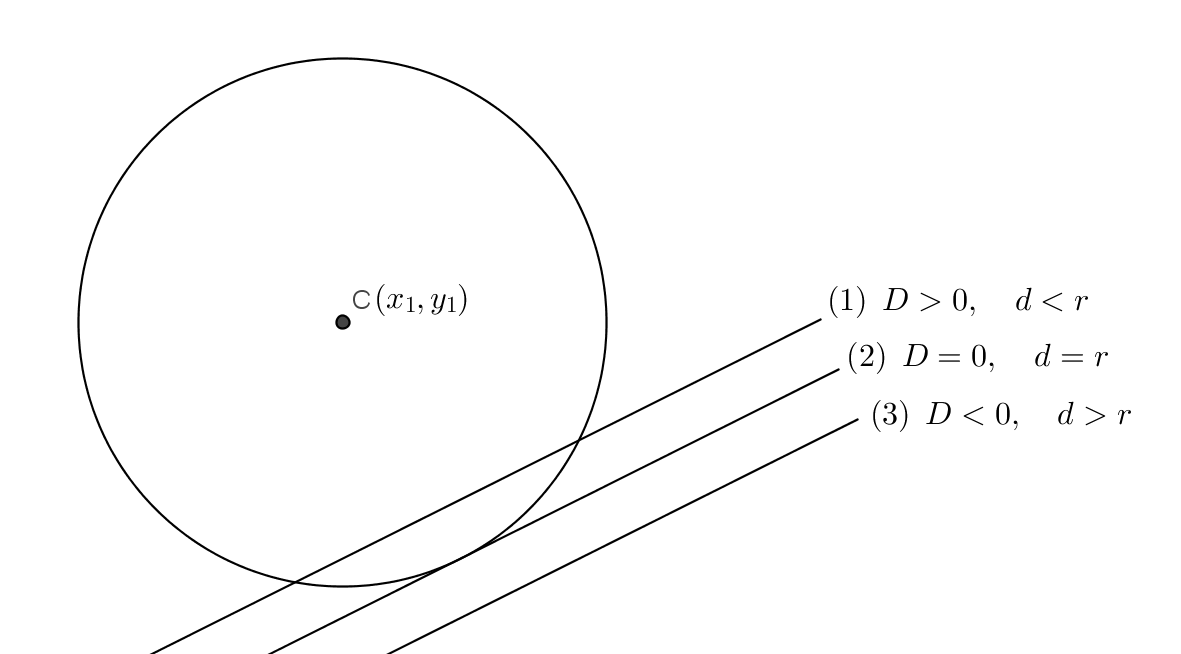
\includegraphics[width=\textwidth]{line-circle}
\caption{원과 직선 사이의 위치 관계}
\label{line-circle}
\end{figure}

%%
\section{도형의 이동}

%
\summ{}
\begin{enumerate}
\item
좌표평면 위의 점 \(P(x,y)\)를
\begin{enumerate}
\item
\(x\)축으로 \(a\)만큼, \(y\)축으로 \(b\)만큼 평행이동 시키면 \((x+a,y+b)\)이 된다.
\item
\(x\)축에 대해 대칭이동시키면 \((x,-y)\)가 된다.
\item
\(y\)축에 대해 대칭이동시키면 \((-x,y)\)가 된다.
\item
원점에 대해 대칭이동시키면 \((-x,-y)\)가 된다.
\item
\(y=x\)에 대해 대칭이동시키면 \((y,x)\)가 된다.
\end{enumerate}
\item
좌표평면 위의 도형 \(f(x,y)=0\)을
\begin{enumerate}
\item
\(x\)축으로 \(a\)만큼, \(y\)축으로 \(b\)만큼 평행이동 시키면 \(f(x-a,y-b)=0\)이 된다.
(\(x\) 대신에 \(x-a\)를 대입하고 \(y\) 대신에 \(y-b\)를 대입한다.)
\item
\(x\)축에 대해 대칭이동시키면 \(f(x,-y)=0\)가 된다.
(\(y\) 대신에 \(-y\)를 대입한다.)
\item
\(y\)축에 대해 대칭이동시키면 \(f(-x,y)=0\)가 된다.
(\(x\) 대신에 \(-x\)를 대입한다.)
\item
원점에 대해 대칭이동시키면 \(f(-x,-y)=0\)가 된다.
(\(x\) 대신에 \(-x\)를 대입하고 \(y\) 대신에 \(-y\)를 대입한다.)
\item
\(y=x\)에 대해 대칭이동시키면 \(f(y,x)=0\)가 된다.
(\(x\) 대신에 \(y\)를 대입하고 \(y\) 대신에 \(x\)를 대입한다.)
\end{enumerate}
\end{enumerate}


%%
\section{부등식의 영역}

%
\summ{}
\begin{enumerate}
\item
함수 \(f\)에 대해 부등식이 나타내는 영역은 다음과 같이 표시된다.
\par
\bigskip
\noindent
{\footnotesize
\begin{tabular}{p{0.24\textwidth}|p{0.24\textwidth}|p{0.24\textwidth}|p{0.24\textwidth}}
\hline
\(y>f(x)\)	&\(y\ge f(x)\)	&\(y< f(x)\)	&\(y\le f(x)\)\\
\hline
\raisebox{-.5\height}{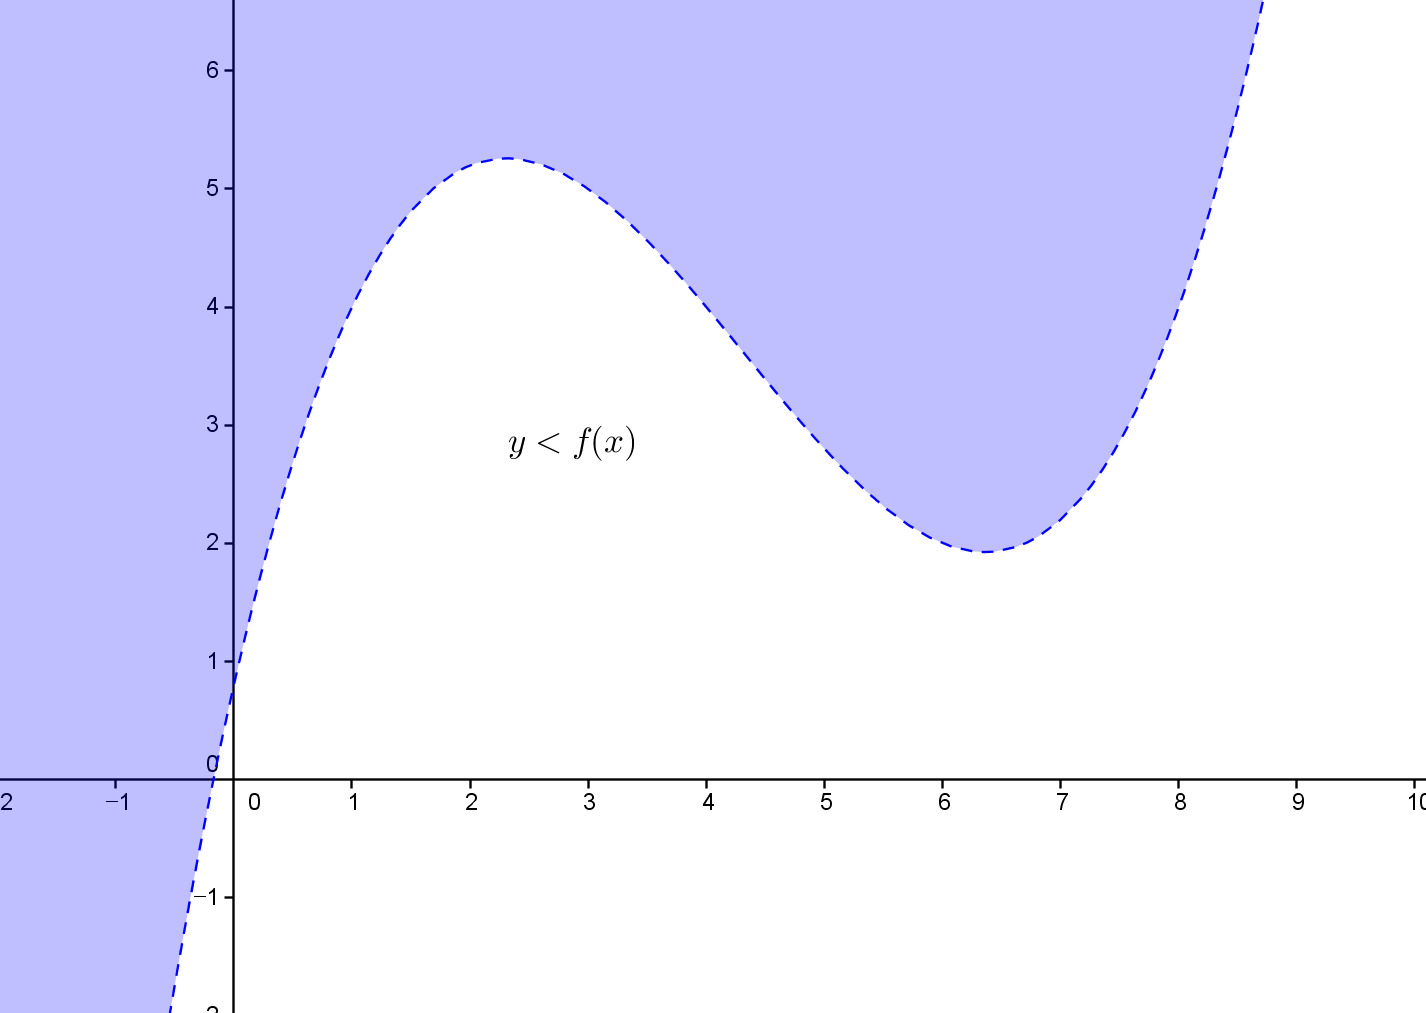
\includegraphics[width=0.24\textwidth]{ineq_1}}
&\raisebox{-.5\height}{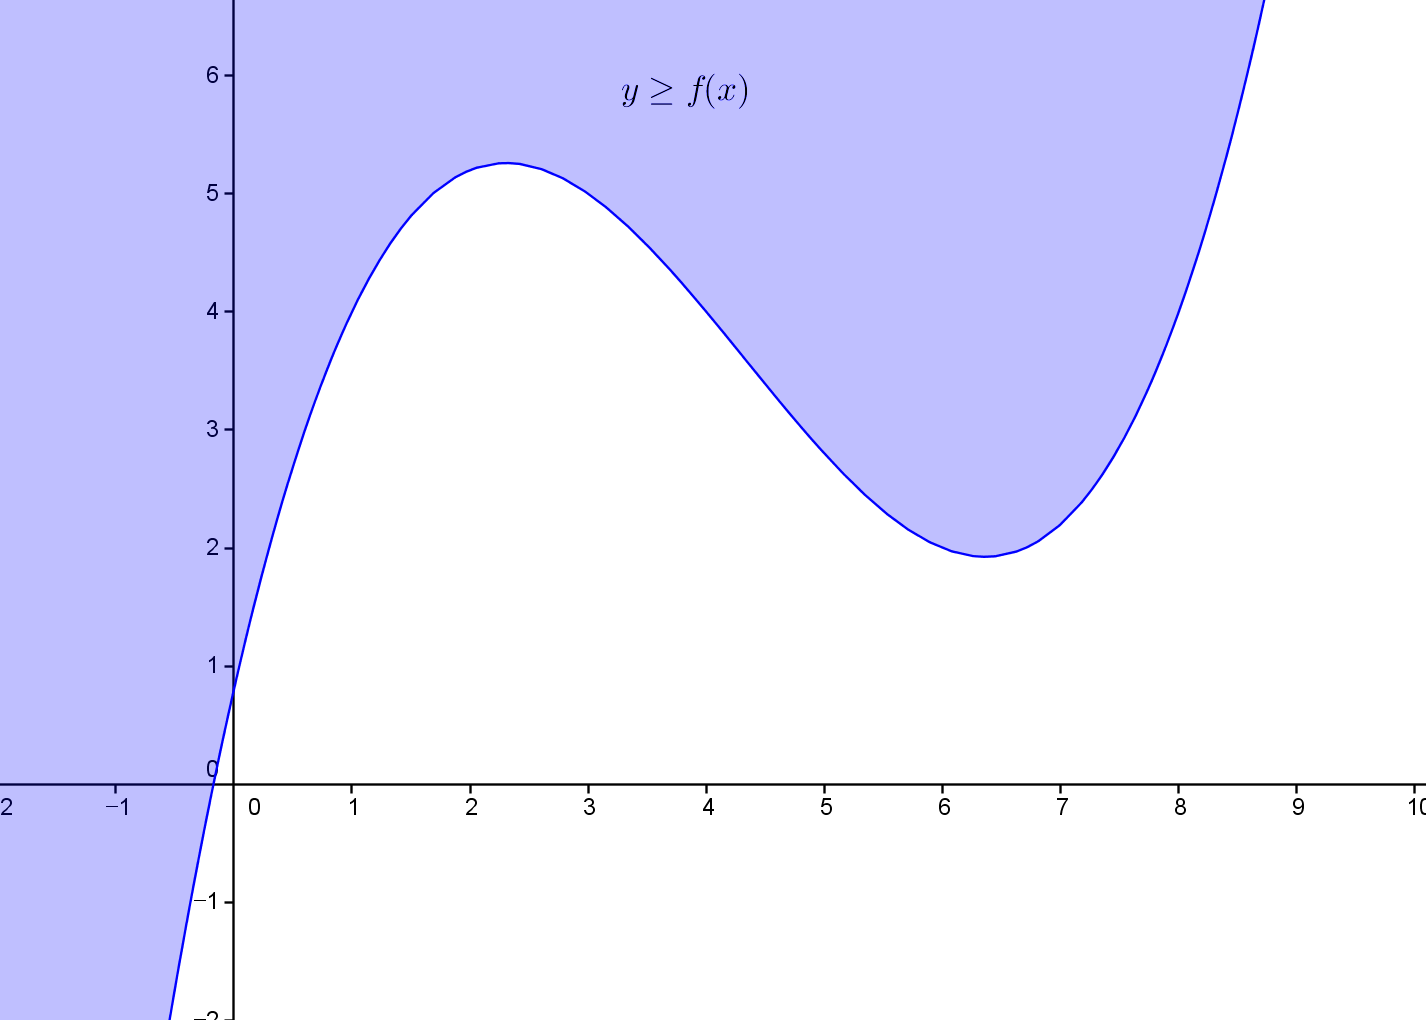
\includegraphics[width=0.24\textwidth]{ineq_2}}
&\raisebox{-.5\height}{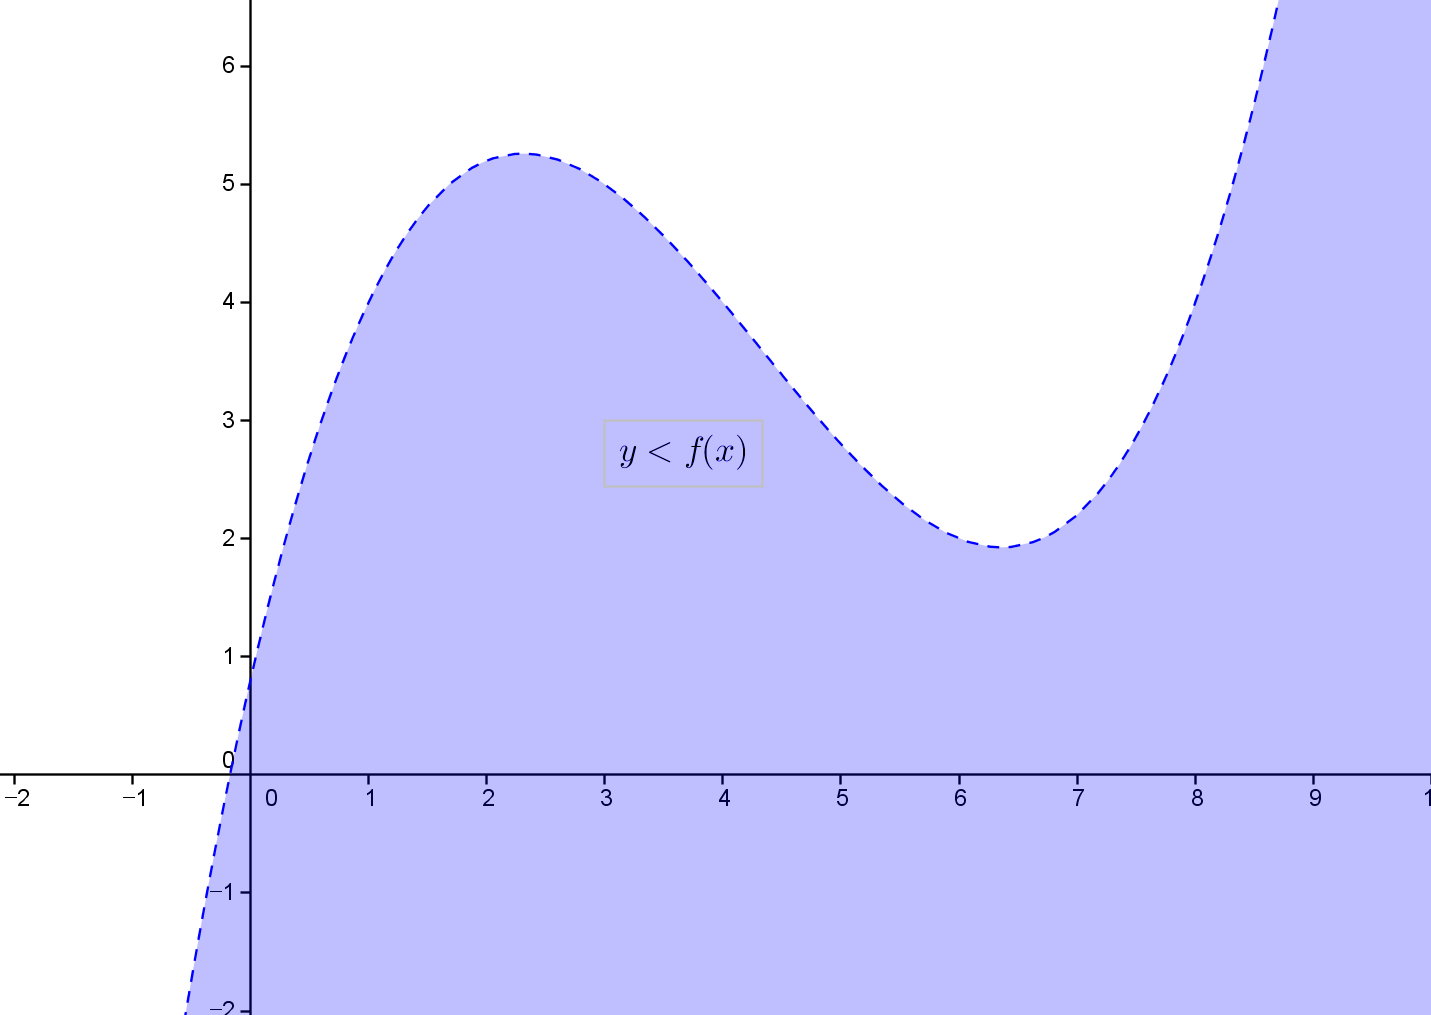
\includegraphics[width=0.24\textwidth]{ineq_3}}
&\raisebox{-.5\height}{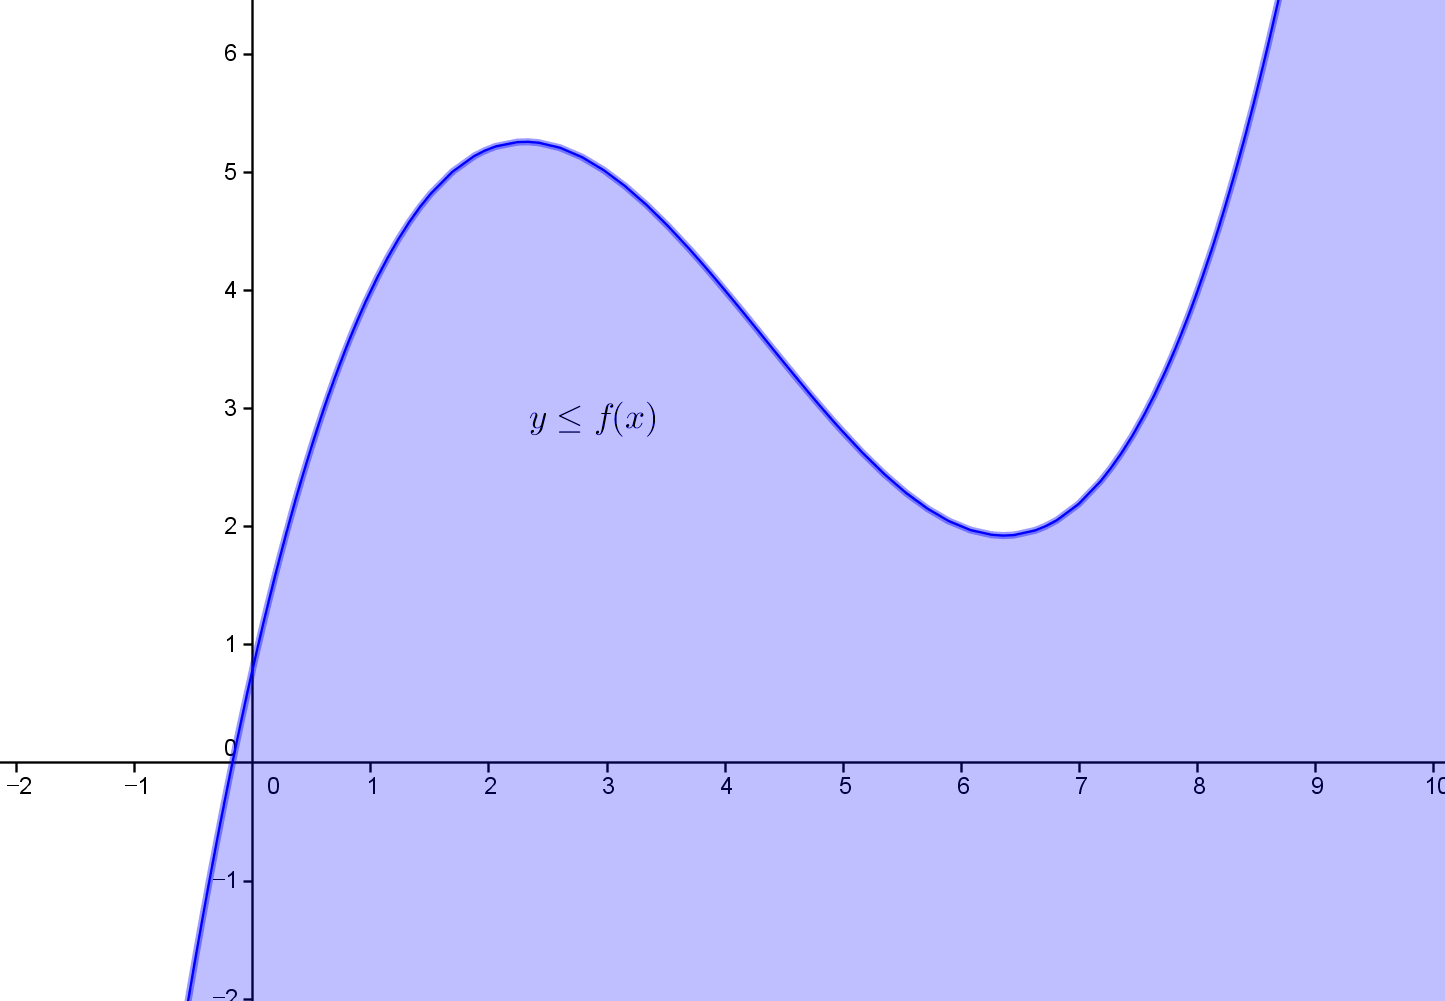
\includegraphics[width=0.24\textwidth]{ineq_4}}
\\\hline
\end{tabular}}
\item
경계선이 원인 경우의 부등식의 영역은 다음과 같이 표시된다.
\par
\bigskip
\noindent
{\footnotesize
\begin{tabular}{p{0.24\textwidth}|p{0.24\textwidth}|p{0.24\textwidth}|p{0.24\textwidth}}
\hline
\(x^2+y^2<r^2\)	&\(x^2+y^2\le r^2\)	&\(x^2+y^2>r^2\)	&\(x^2+y^2\ge r^2\)\\
\hline
\raisebox{-.5\height}{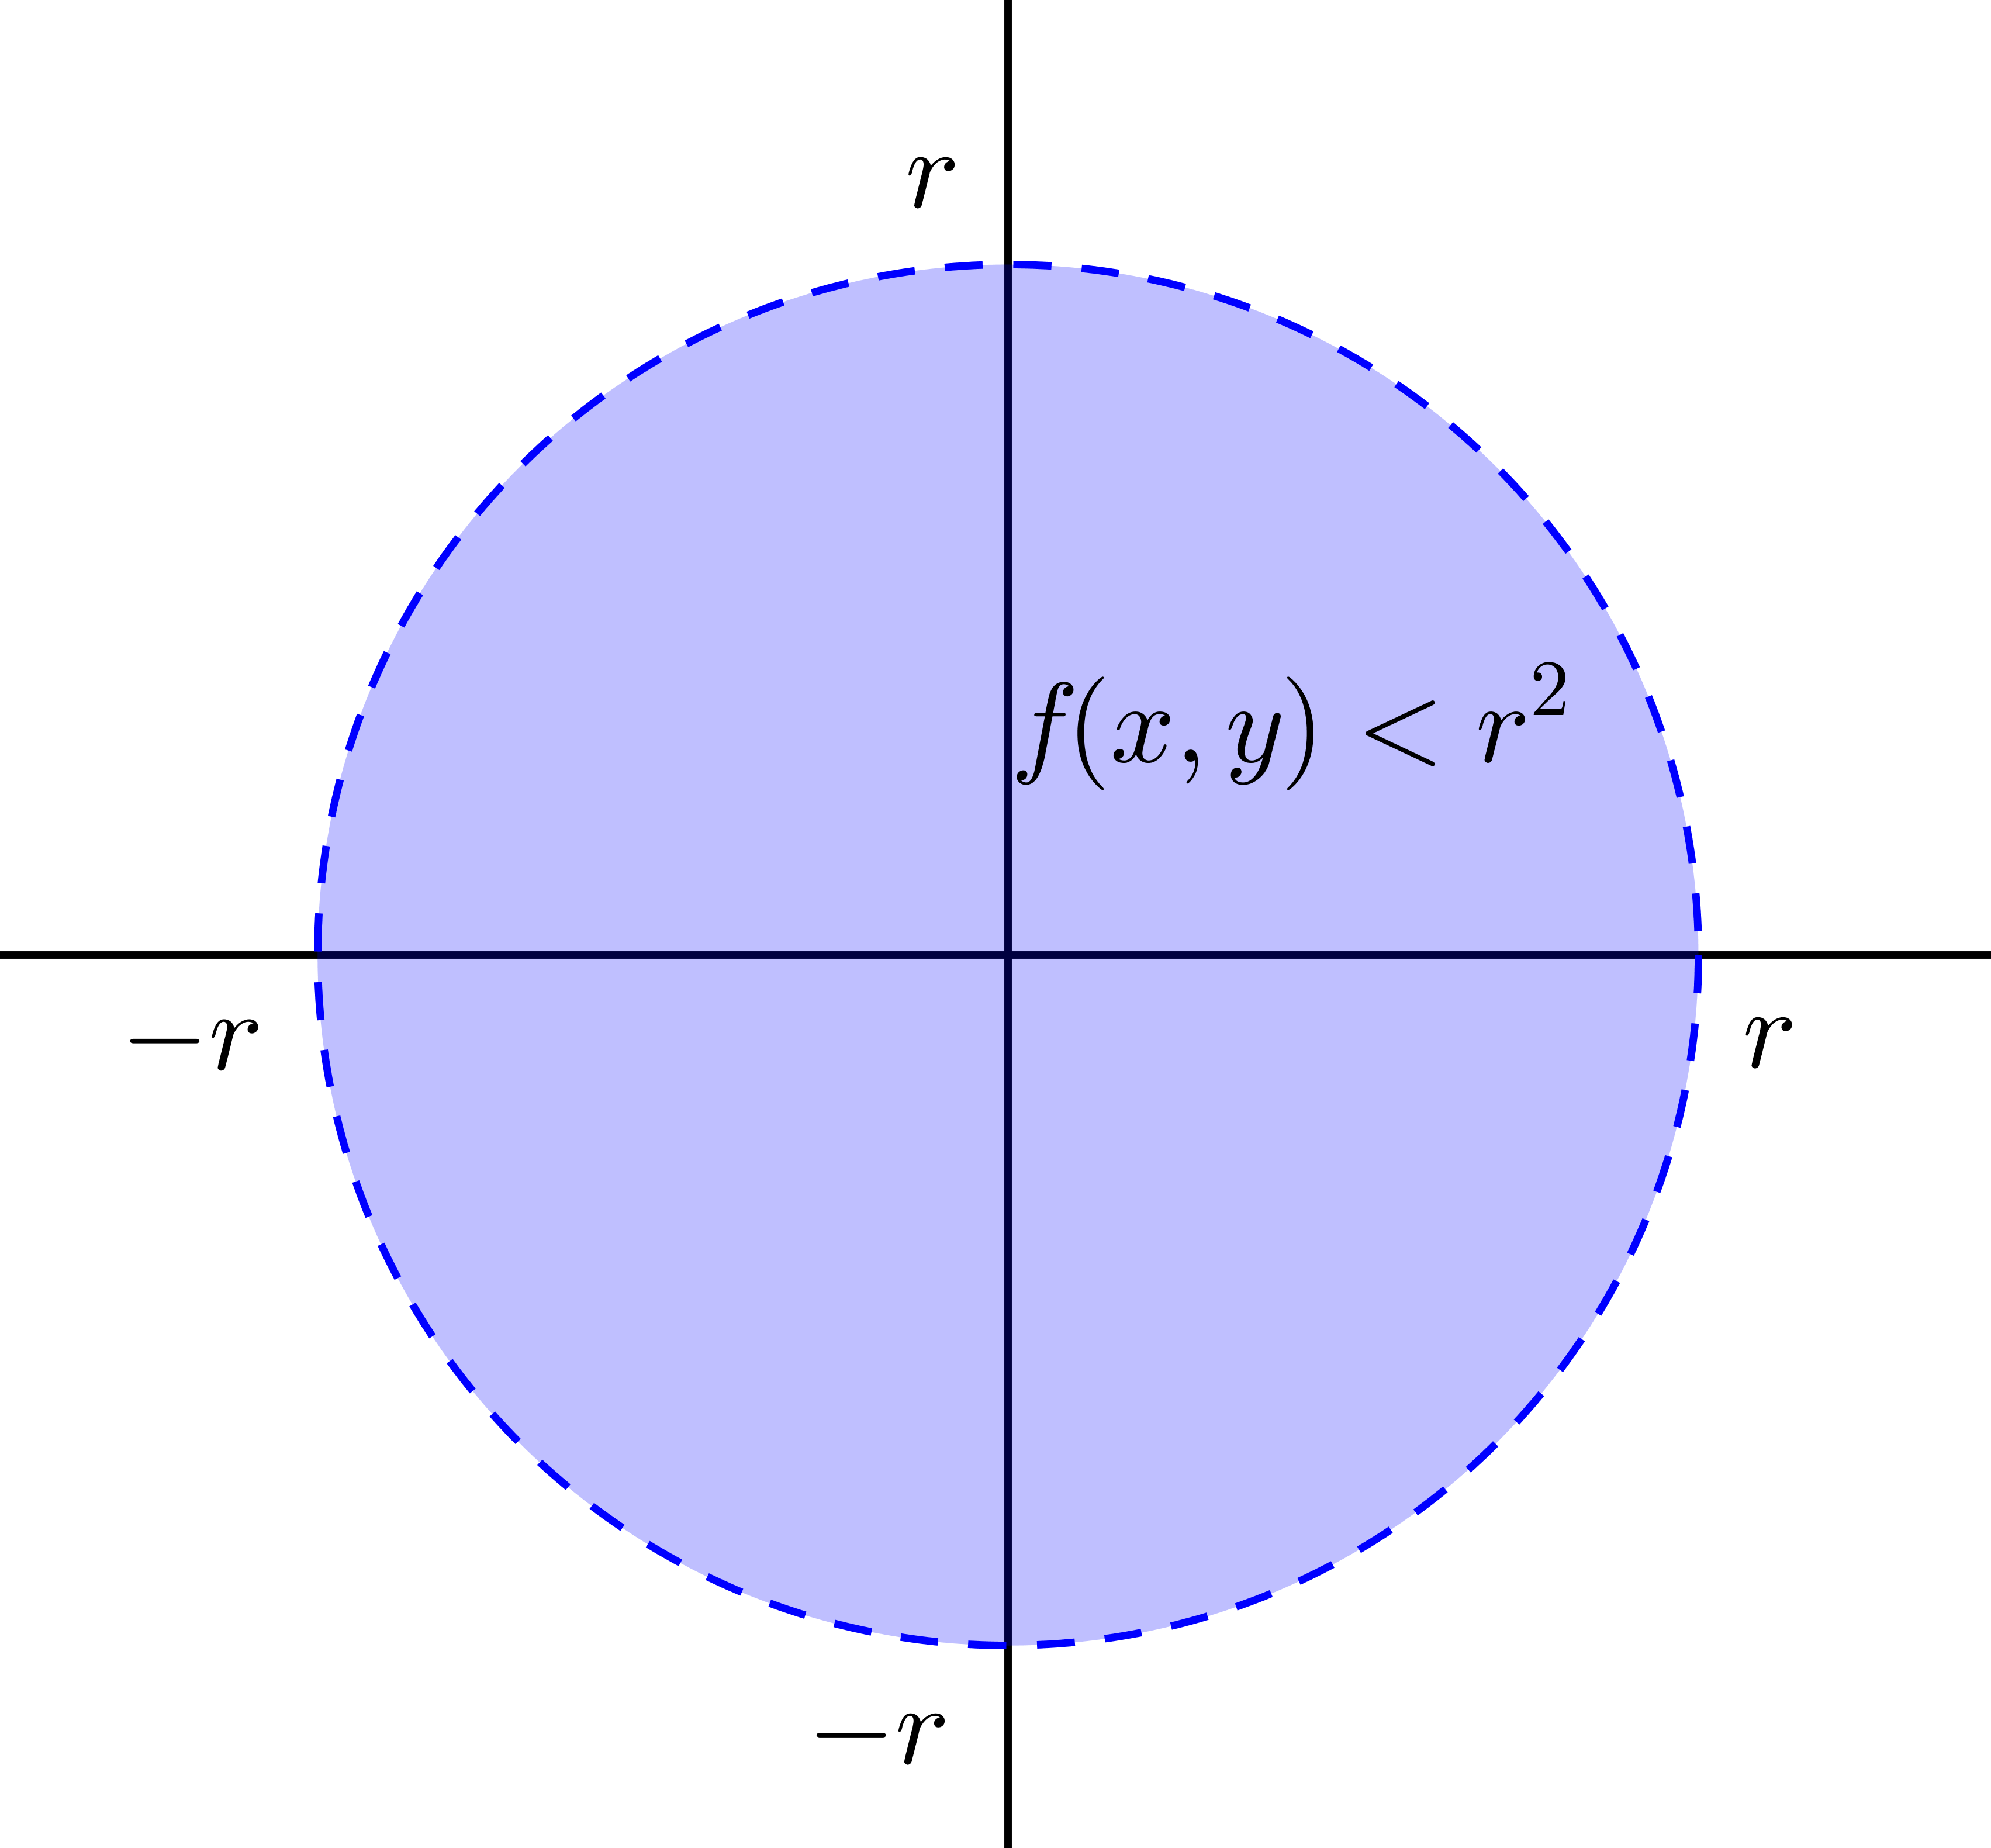
\includegraphics[width=0.24\textwidth]{ineq_circ_1}}
&\raisebox{-.5\height}{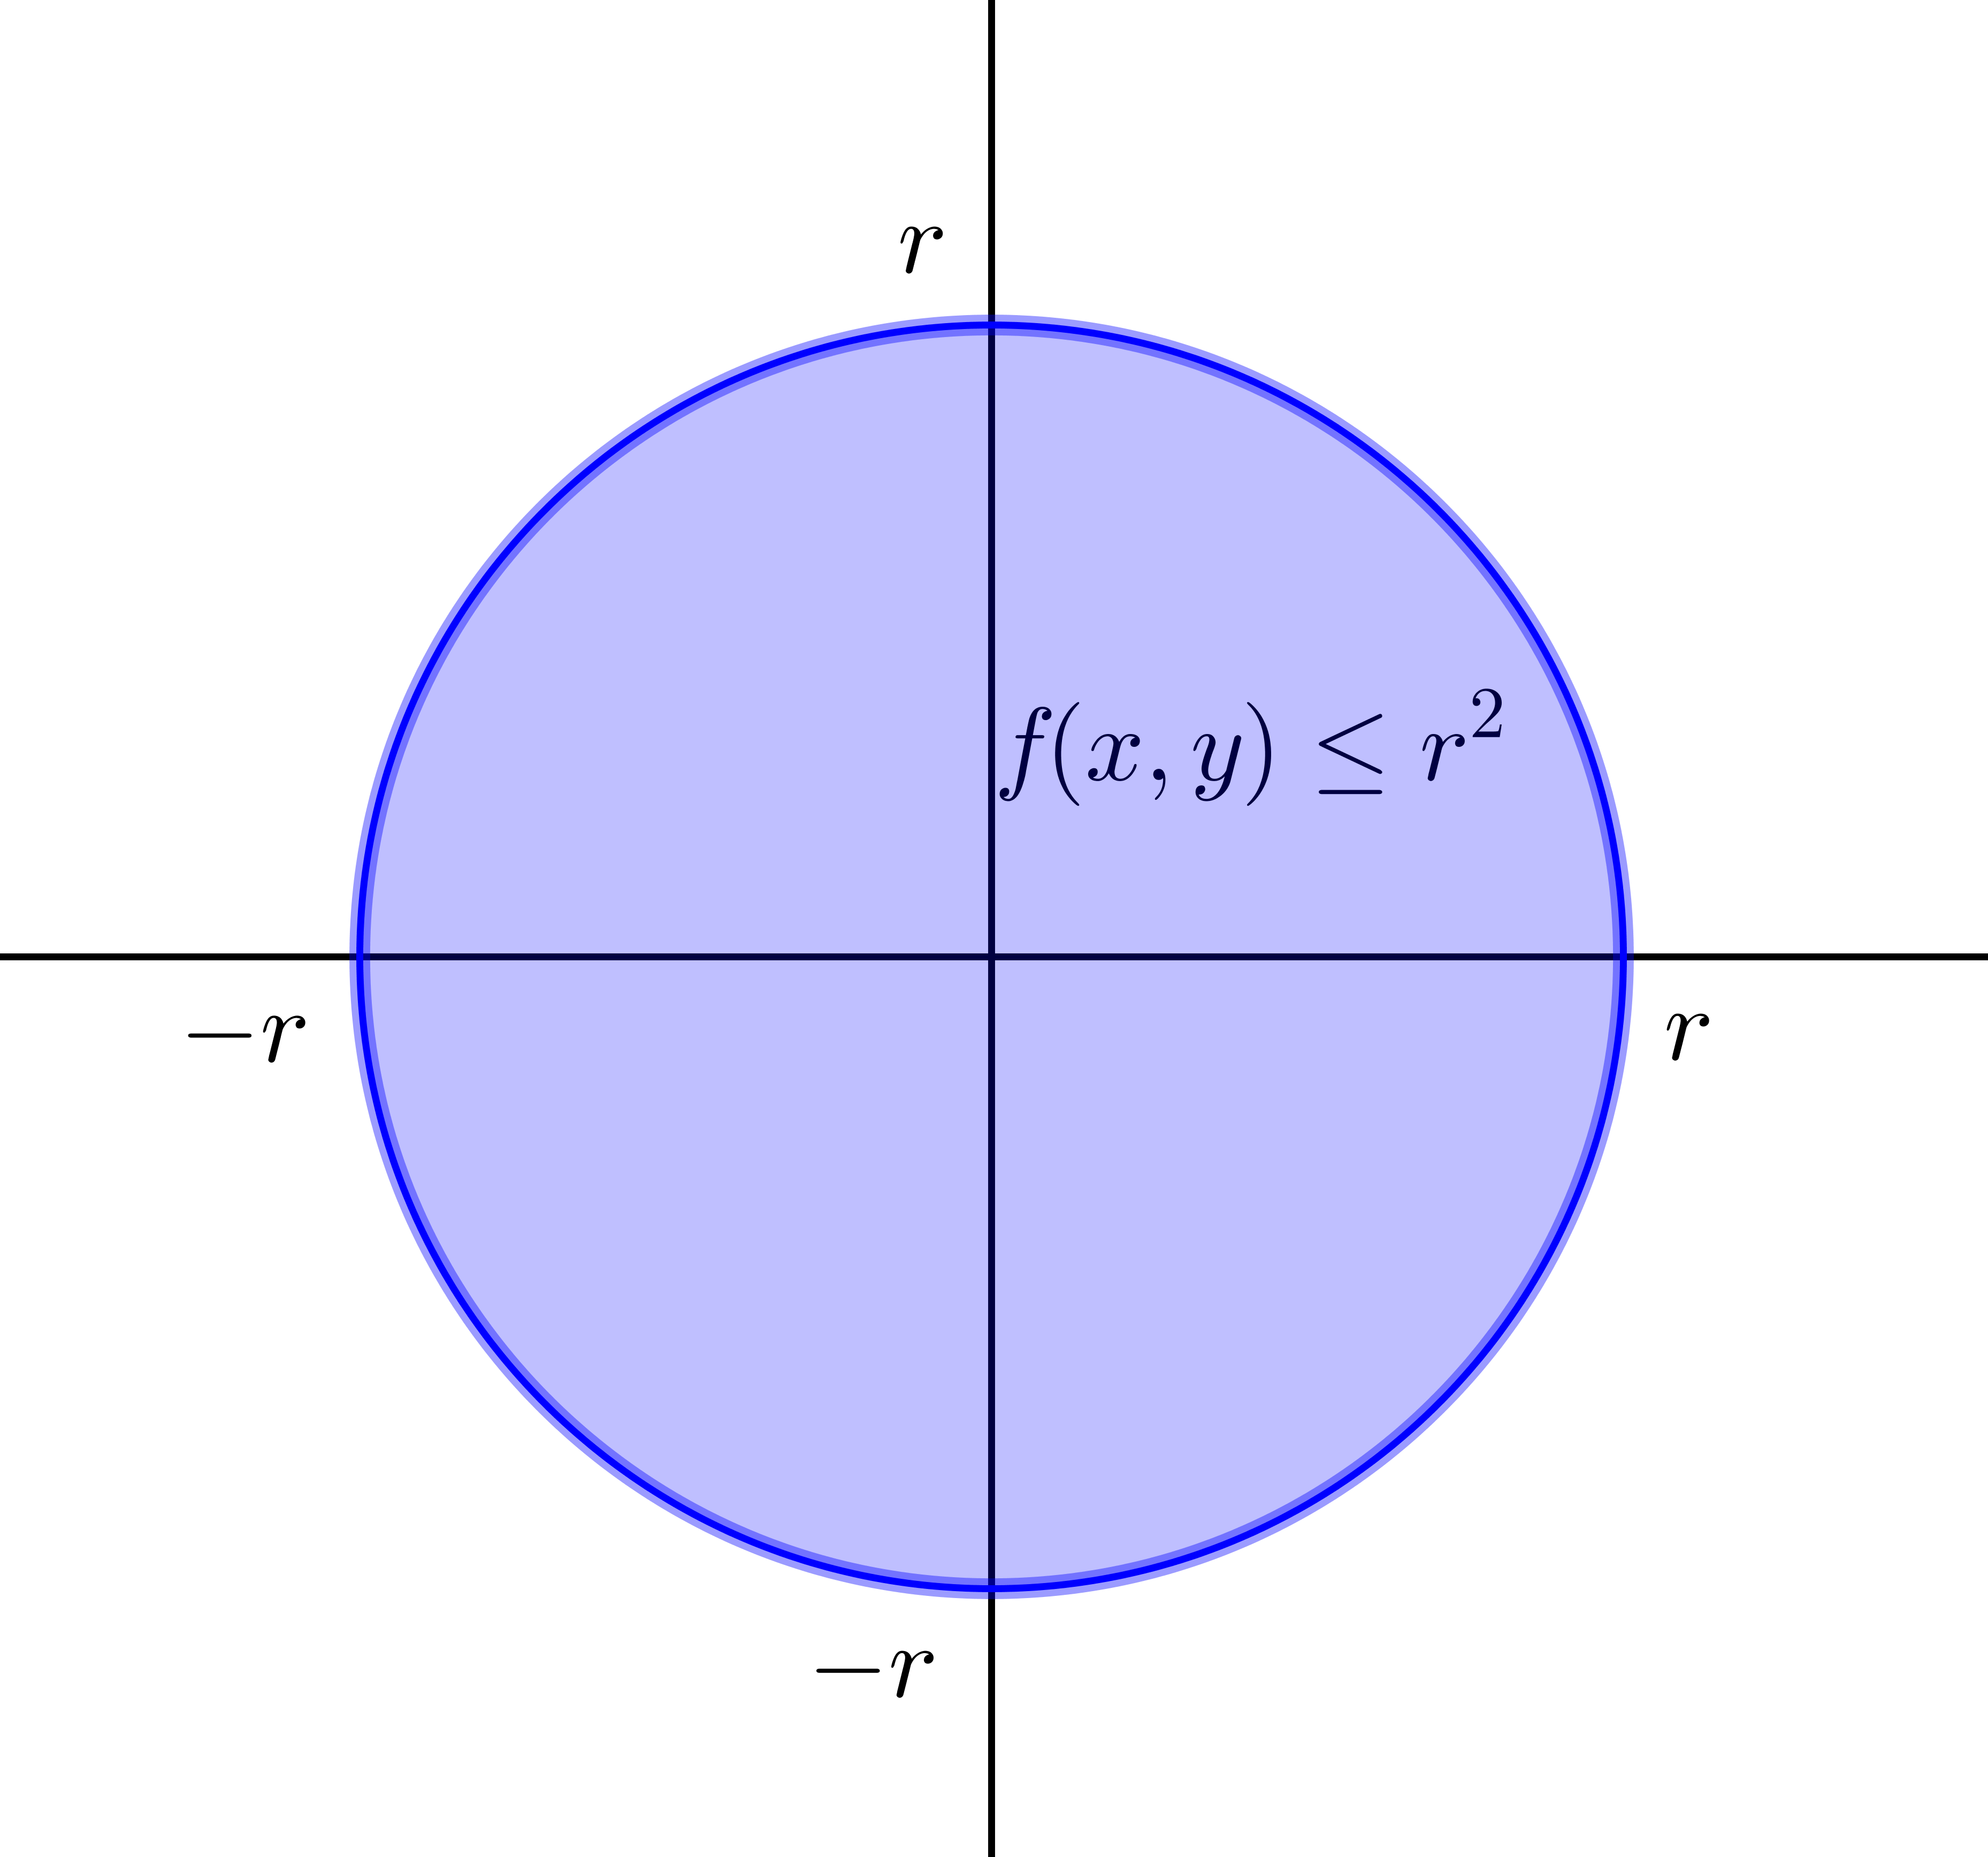
\includegraphics[width=0.24\textwidth]{ineq_circ_2}}
&\raisebox{-.5\height}{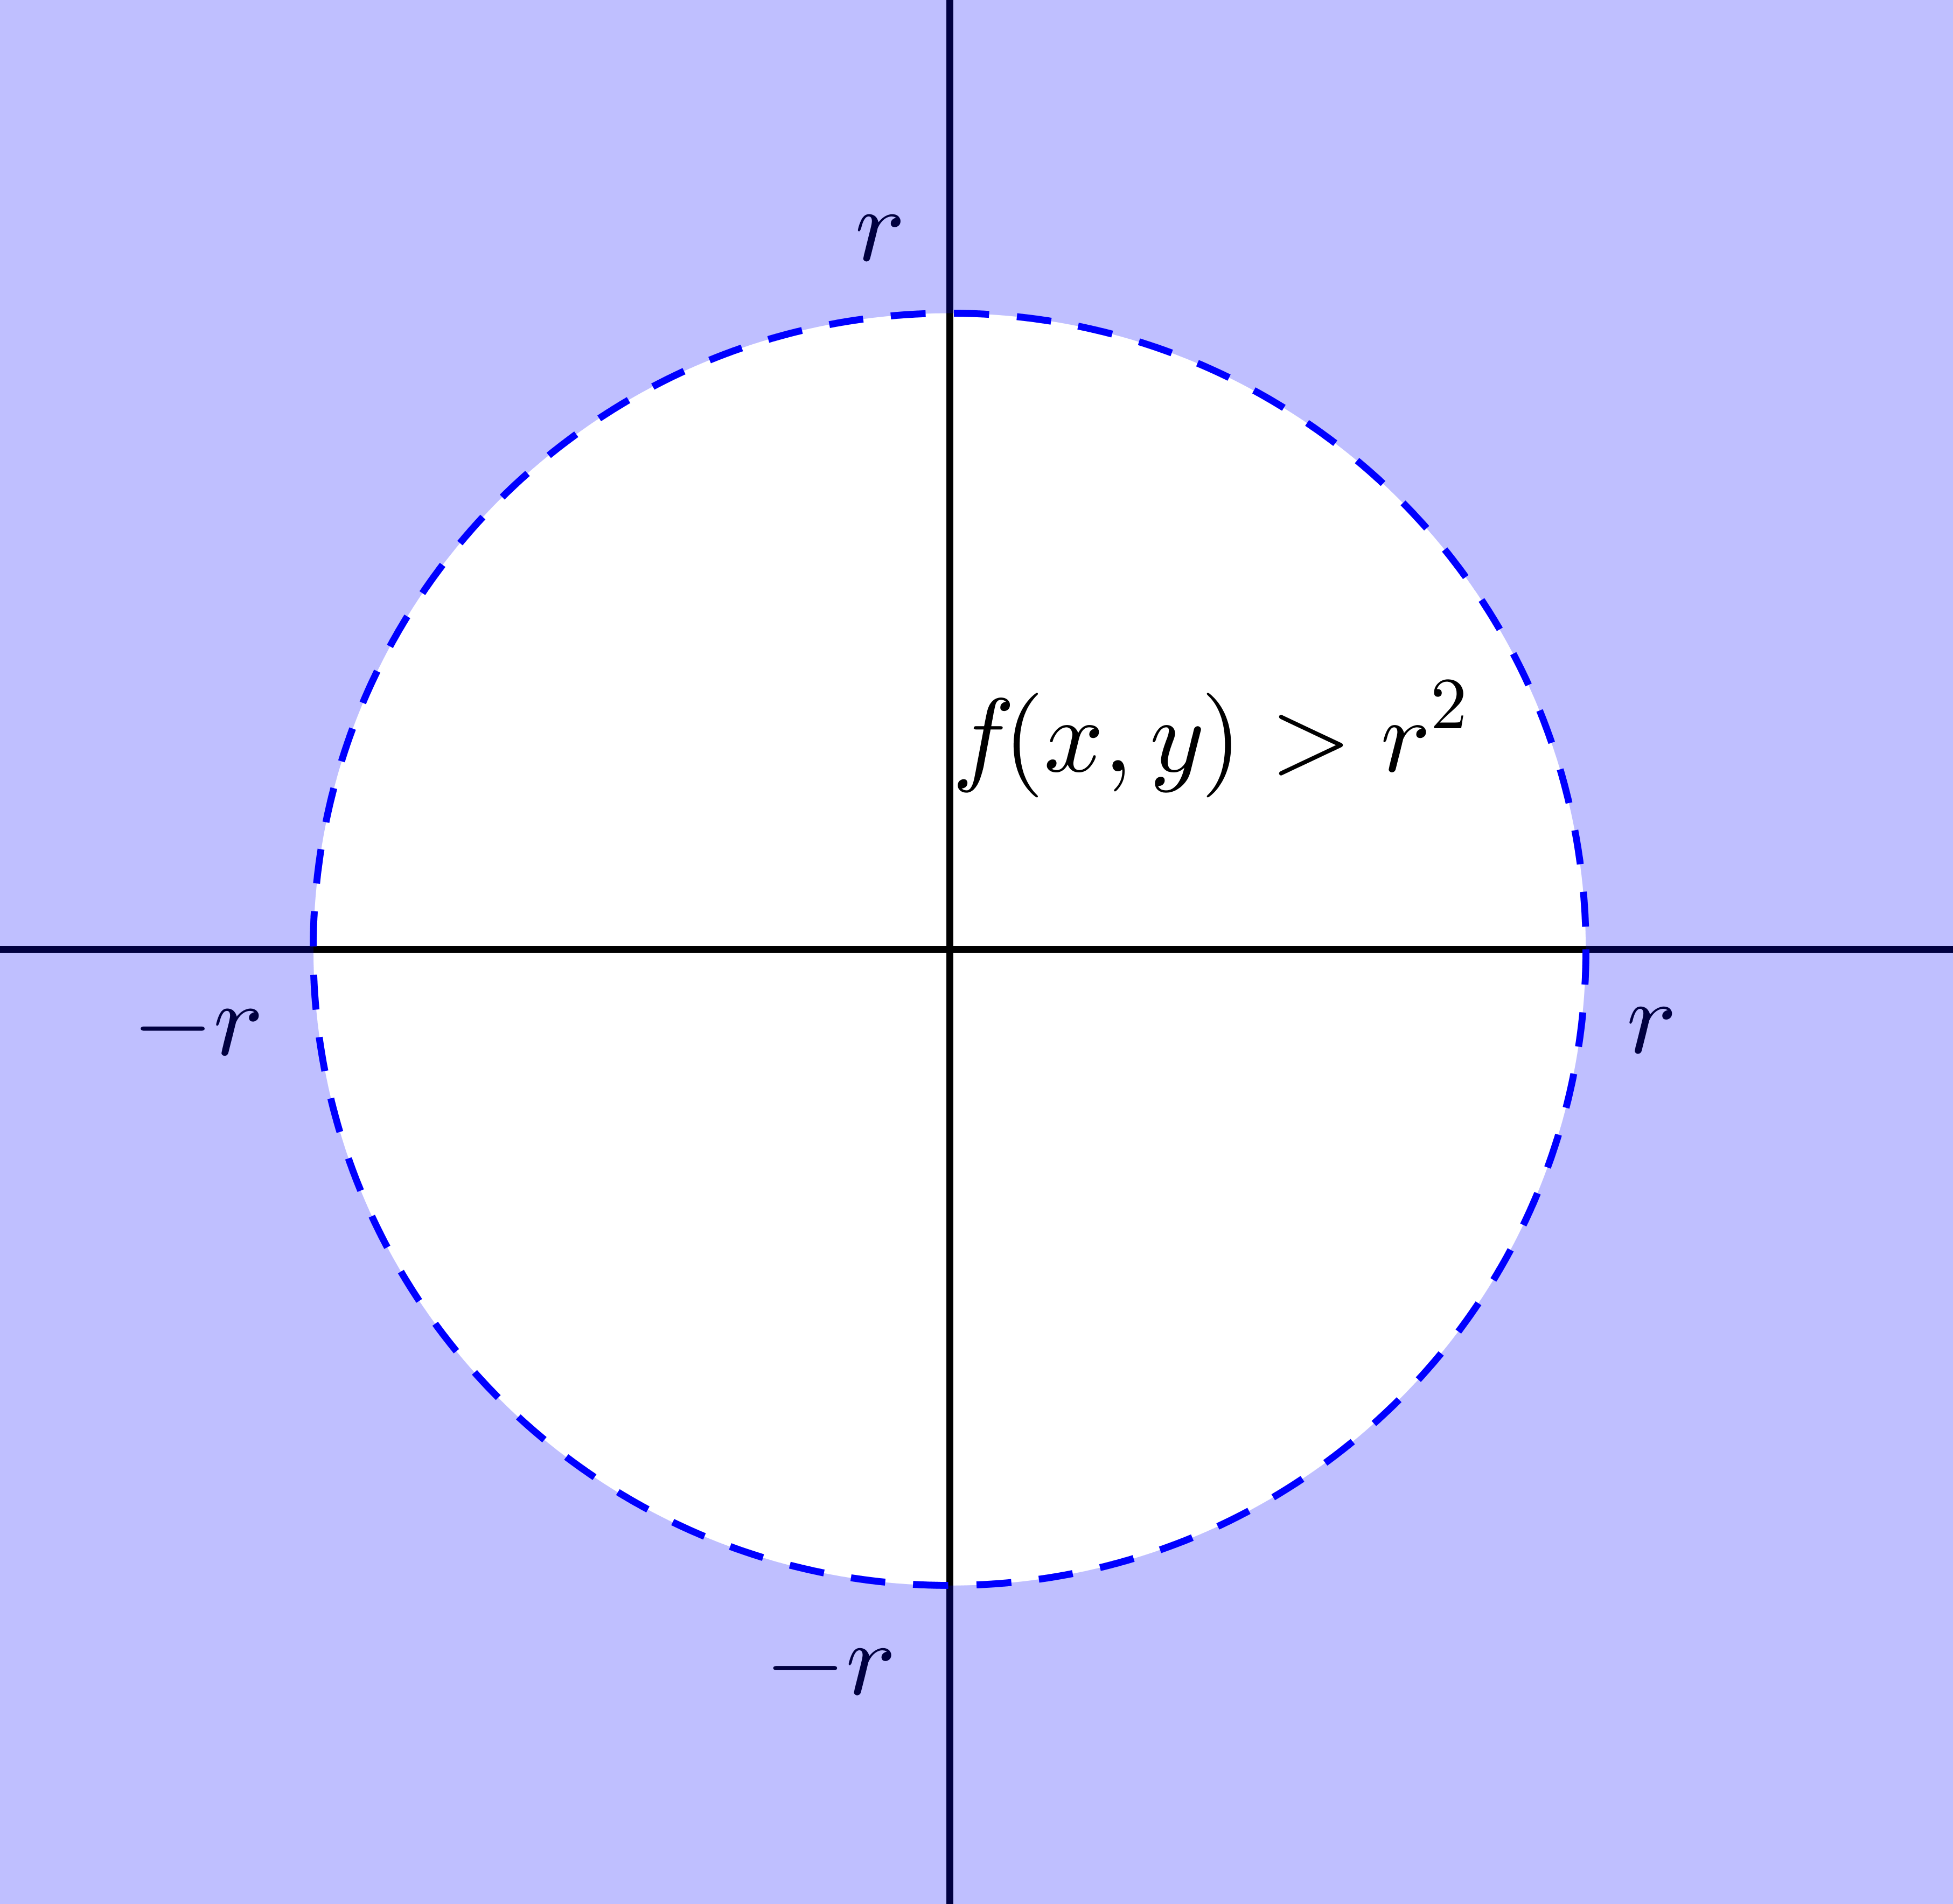
\includegraphics[width=0.24\textwidth]{ineq_circ_3}}
&\raisebox{-.5\height}{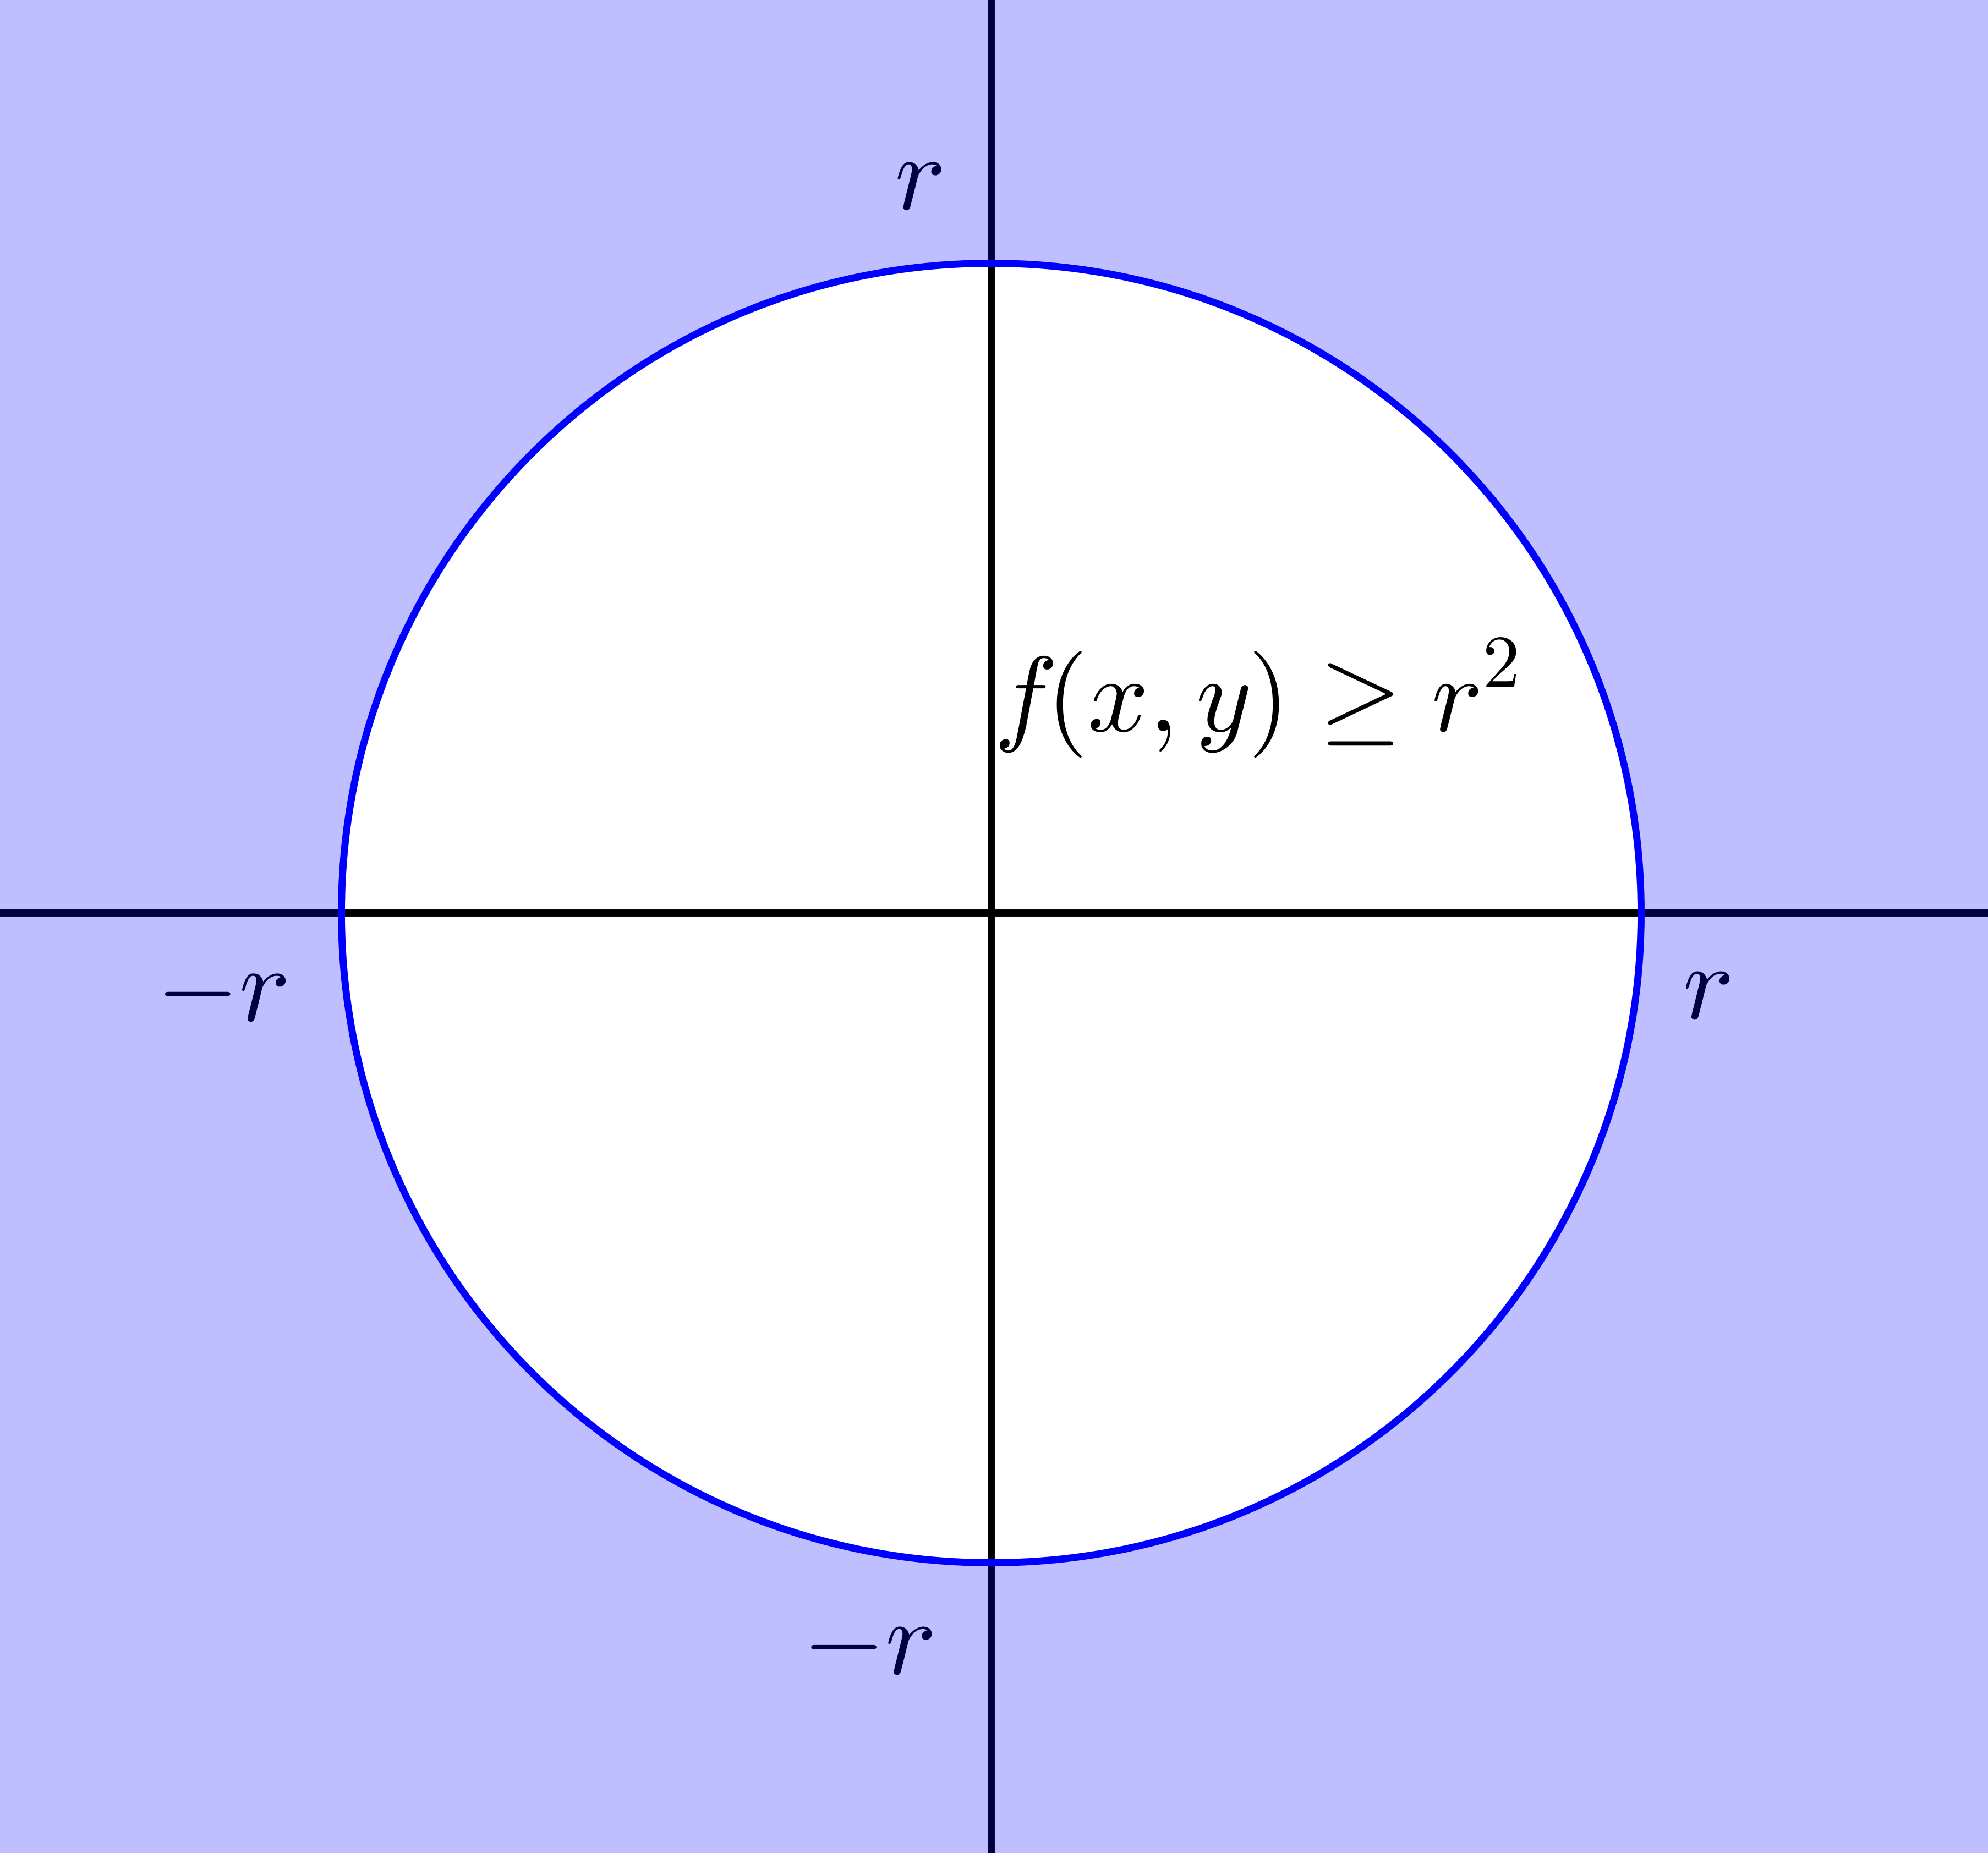
\includegraphics[width=0.24\textwidth]{ineq_circ_4}}
\\\hline
\end{tabular}}
\item
연립부등식의 경우, 두 부등식의 영역이 겹쳐지는 부분이 연립 부등식의 영역이다.
\end{enumerate}




\end{document}